\title[Causality]{Causality: Lecture 10}
\author[Joris Mooij]{\\[5mm]\large Joris Mooij \& Patrick Forr\'e\\
\url{j.m.mooij@uva.nl}, \url{p.d.forre@uva.nl}}
\institute[UvA]{University of Amsterdam}
\date[2025-04-10]{\normalsize April 10th, 2025}
\maketitle


\part{Equivalence Relations}
\frame{\partpage}

\begin{comment}
\begin{frame}{Equivalence relations}
Equivalence relations capture the notion that mathematical objects can be ``equivalent'' from some point of view.
\begin{Def}
  Let $Z$ be a set and $R \subseteq Z^2$ be a relation on $Z$ (i.e., a subset of ordered pairs of $Z$). $R$ is called an \emph{equivalence relation} if 
  \begin{enumerate}
    \item $R$ is reflexive: $(a,a) \in R$ for all $a \in Z$;
    \item $R$ is symmetric: $(a,b) \in R \iff (b,a) \in R$ for all $a,b \in Z$;
    \item $R$ is transitive: if $(a,b) \in R$ and $(b,c) \in R$ then $(a,c) \in R$ for all $a,b,c\in Z$.
  \end{enumerate}
\end{Def}
\end{frame}
\end{comment}

\begin{frame}{Equivalence of iSCMs}
  \begin{Def}[\ref{def:equivalent_scms}]
  Let $M = \lt \Sin, \Send, \Srnd, \CX, P, f \rt$ and
  $\tilde{M} = \ltuple \Sin, \Send, \Srnd, \CX, P, \tilde{f} \rtuple$ be two iSCMs.
  We say that
  $M$ is \emph{equivalent} to $\tilde{M}$ and write $M \equiv \tilde{M}$ if for each $v \in \Send$,
  $$x_v = f_v(\xJ,\xV,\xW) \iff x_v = \tilde{f}_v(\xJ,\xV,\xW)\quad M\as.$$
%  In words, $M$ and $\tilde{M}$ are considered equivalent if they at most differ in terms of their
%  causal mechanisms, yet each of their structural equations has the same solutions.
\end{Def}
\begin{Prp}[\ref{prp:equivalent_scms}]
\begin{enumerate}
  \item Equivalence of iSCMs is preserved by interventions (hard, soft, and adding intervention nodes).
  \item Equivalent iSCMs have the same null sets, and `$M\as$' means the same as `$\tilde{M}\as$'.
  \item Equivalent iSCMs have the same potential outcomes, solutions, Markov kernels, and (partial) solution functions.
  \item (Essentially unique) (partial) solvability, essential uniqueness of (partial) solution functions, and simplicity are invariants under iSCM equivalence.
%  \item Essential linearity is preserved under iSCM equivalence.
\end{enumerate}
\end{Prp}
\end{frame}

\begin{frame}{Example}
\begin{Eg}
  Is the SCM with the single structural equation
  $$X = -X^3 + X + W$$
  where $X$ is endogenous, and $W$ is exogenous, equivalent to the SCM obtained by replacing the structural equation with
  $$X = \sqrt[3]{W}$$
  (note that $X$ no longer appears on the r.h.s.)?

  \bigskip
  \uncover<2- |handout:0>{Yes, it is!}
\end{Eg}
\end{frame}

\begin{frame}{Example}
\begin{Eg}
  Is the SCM with endogenous variable $X \in \RN$ and exogenous random variable $W \in \RN$ and structural equation
  $$X = W X + c$$
  equivalent to the SCM obtained by replacing the structural equation with
  $$X = \begin{cases}
          \xi & W = 1 \\
          \frac{c}{1 - W} & W \ne 1
        \end{cases}$$
  for some choice of $\xi \in \RN$ and $P(W)$?

  \bigskip
  \uncover<2- |handout:0>{This depends on $P(W)$. If $P(W=1)=0$, then yes, otherwise no. The value of $\xi$ is irrelevant.}
\end{Eg}
%  \uncover<2- |handout:0>{If one does not model interventions on exogenous random variables (like e.g.\ Pearl), weaker notions of equivalence can be used (see \cite{BFPM21}).}
\end{frame}

\begin{frame}{Observational and interventional equivalence ($J=\emptyset$)}
  \begin{Def}[SCMs]
  Let $M = \lt \Sin, \Send, \Srnd, \CX, P, f \rt$ and
  $\tilde{M} = \ltuple \tilde{\Sin}, \tilde{\Send}, \tilde{\Srnd}, \tilde{\CX}, \tilde{P}, \tilde{f} \rtuple$ be two simple SCMs
  (that is, $J = \tilde{J} = \emptyset$) and $O \subseteq \Send \cap \tilde{\Send}$ a common subset.

  We say that:
  \begin{enumerate}
    \item $M$ and $\tilde{M}$ are \emph{observationally equivalent w.r.t.\ $O$} if $\CX_O = \tilde{\CX}_O$ and their marginal distributions coincide:
      $$P_{M}(X_O) = P_{\tilde{M}}(X_O).$$
    \item $M$ and $\tilde{M}$ are \emph{interventionally equivalent w.r.t.\ $O$} if for every subset $T \subseteq O$ the intervened iSCMs $M_{\doit(T)}$ and $\tilde{M}_{\doit(T)}$ are observationally equivalent w.r.t.\ $O \setminus T$.
%    \item $M$ and $\tilde{M}$ are said to be \emph{counterfactually equivalent w.r.t.\ $O$} if the twin iSCMs $M^\twin$ and $\tilde{M}^\twin$ are interventionally equivalent w.r.t.\ $O \cup O'$, where $O'$ is the copy of $O$ in $\Send' \cap \tilde{\Send}'$.
  \end{enumerate}
\end{Def}
Generalizing this to exogenous inputs nodes leads us to\dots
\end{frame}

\begin{frame}{Observable and interventional equivalence}
  \begin{Def}[\ref{def:scm_obs_interv_equiv}]
  Let $M = \lt \Sin, \Send, \Srnd, \CX, P, f \rt$ and
  $\tilde{M} = \ltuple \tilde{\Sin}, \tilde{\Send}, \tilde{\Srnd}, \tilde{\CX}, \tilde{P}, \tilde{f} \rtuple$ be two simple iSCMs
  and $O \subseteq \Send \cap \tilde{\Send}$ a common subset.
  We say that:
  \begin{enumerate}
    \item $M$ and $\tilde{M}$ are \emph{observably equivalent w.r.t.\ $O$} if $\CX_O = \tilde{\CX}_O$, $\CX_{J \cap \tilde{J}} = \tilde{\CX}_{J \cap \tilde{J}}$ and their marginal Markov kernels coincide:
      $$P_{M}(X_O \mid \doit(X_J)) = P_{\tilde{M}}(X_O \mid \doit(X_{\tilde J})).$$
    This has to be interpreted as both Markov kernels being a version of a Markov kernel $\CX_{J \cap \tilde{J}} \dshto \CX_O$,
    i.e., $P_{M}(X_O \mid \doit(X_J))$ must be constant in $x_{J \setminus \tilde{J}}$ and
    $P_{\tilde{M}}(X_O \mid \doit(X_{\tilde{J}}))$ must be constant in $x_{\tilde{J} \setminus J}$;
%    \item $M$ and $\tilde{M}$ are \emph{observably equivalent w.r.t.\ $O$} if $\CX_O = \tilde{\CX}_O$, $J = \tilde{J}$, $\CX_J = \tilde{\CX}_J$ and $P_{M}(X_O \mid \doit(\XJ)) = P_{\tilde{M}}(X_O \mid \doit(\XJ))$;
    \item $M$ and $\tilde{M}$ are \emph{interventionally equivalent w.r.t.\ $O$} if for every subset $T \subseteq O$ the intervened iSCMs $M_{\doit(T)}$ and $\tilde{M}_{\doit(T)}$ are observably equivalent w.r.t.\ $O \setminus T$.
%    \item $M$ and $\tilde{M}$ are said to be \emph{counterfactually equivalent w.r.t.\ $O$} if the twin iSCMs $M^\twin$ and $\tilde{M}^\twin$ are interventionally equivalent w.r.t.\ $O \cup O'$, where $O'$ is the copy of $O$ in $\Send' \cap \tilde{\Send}'$.
  \end{enumerate}
\end{Def}
\end{frame}

\begin{frame}{A note on terminology}
%  I changed:
%  \begin{itemize}
%    \item `observationally equivalent' $\mapsto$ `observably equivalent', and
%    \item `observational equivalence' $\mapsto$ `observable equivalence'
%  \end{itemize}
%  throughout the second part of the lecture notes.
%
%  \bigskip
  In the definition of observable equivalence, we deviate slightly from common terminology.

  \bigskip
  \begin{description}
    \item[observational] non-experimental (in the absence of any intervention),\\
      e.g., `observational data', `observational distribution'
    \item[observable] something that can be measured (the opposite of latent),\\
      e.g., `observable variable'
    \item[observed] something that has been measured,\\
      e.g., `observed variable'
  \end{description}

  \bigskip
  Therefore we also speak of `observational equivalence' as a synonym for observable equivalence in case $J \cap \tilde{J} = \emptyset$.
\end{frame}

\begin{frame}{Relationships between equivalences}
  \begin{Rem}[\ref{rem:scm_interv_equiv}]
  Note that $M$ and $\tilde{M}$ are interventionally equivalent w.r.t.\ $O \ins (V \cap \tilde{V})$ if and only if
  $\CX_O = \tilde{\CX}_O$, $\CX_{J \cap \tilde{J}} = \tilde{\CX}_{J \cap \tilde{J}}$
  and for all $T \ins O$:
    $$P_{M}(X_O \mid \doit(X_J,X_T)) = P_{\tilde{M}}(X_O \mid \doit(X_{\tilde J},X_T)).$$
\end{Rem}
The equivalence relations form a hierarchy:
  \begin{Prp}[\ref{prp:pearls_ladder_levels_1_and_2}]
  For simple iSCMs $M, \tilde{M}$ and a subset $O \subseteq \Send \cap \tilde{\Send}$:
  \begin{enumerate}
    \item If $M \equiv \tilde{M}$ then $M$ and $\tilde{M}$ are interventionally equivalent w.r.t.\ $O$.
    \item Interventional equivalence of $M$ and $\tilde{M}$ w.r.t.\ $O$ implies observable equivalence of $M$ and $\tilde{M}$ w.r.t.\ $O$.
  \end{enumerate}
\end{Prp}
The reverse implication of the second item does not hold in general. 
This expresses that causal modeling is more refined than probabilistic modeling.
\end{frame}

\begin{frame}{Example}
\begin{Eg}
  The following SCMs are both simple:
  \begin{align*}
    M &: \qquad W \sim \C{N}(\mu,\sigma^2) \qquad N = W, C = \alpha + \beta N \\
    \tilde{M}&: \qquad W \sim \C{N}(\tilde{\mu},\tilde{\sigma}^2) \qquad C = W, N = \tilde{\alpha} + \tilde{\beta} C
  \end{align*}
Their distributions are respectively 
  $$P_M\left(\begin{pmatrix}N \\C\end{pmatrix}\right) = \C{N}\left(\begin{pmatrix} \mu \\ \alpha + \beta \mu \end{pmatrix}, \begin{pmatrix} \sigma^2 & \beta\sigma^2 \\ \beta\sigma^2 & \beta^2\sigma^2\end{pmatrix}\right)$$
and
  $$P_{\tilde{M}}\left(\begin{pmatrix}N\\C\end{pmatrix}\right) = \C{N}\left(\begin{pmatrix} \tilde{\alpha} + \tilde{\beta}\tilde{\mu} \\ \tilde{\mu} \end{pmatrix}, \begin{pmatrix} \tilde{\beta}^2\tilde{\sigma}^2 & \tilde{\beta}\tilde{\sigma}^2 \\ \tilde{\beta}\tilde{\sigma}^2 & \tilde{\sigma}^2\end{pmatrix}\right)$$
For which parameters are they observably equivalent (w.r.t.\ $\{N,C\}$)?\\
For which parameters are they interventionally equivalent (w.r.t.\ $\{N,C\}$)?
\end{Eg}
\end{frame}

\begin{frame}{Is interventional equivalence preserved under interventions?}
Equivalence was preserved under interventions. 
This is also the case for interventional equivalence (although one has to be careful with respect to which subset).
\begin{Prp}[\ref{prp:scm_interventions_preserve_interv_equiv}]
  Assume that $M$ and $\tilde{M}$ are interventionally equivalent iSCMs w.r.t.\ $O \ins (V \cap \tilde{V})$. Then, for $T \subseteq O \cup (J \cap \tilde{J})$:
    \begin{enumerate}
      \item $M_{\doit(T)}$ and $\tilde{M}_{\doit(T)}$ are interventionally equivalent w.r.t.\ $O \sm T$ (hard interventions with unspecified target value);
      \item $M_{\doit(X_T=\xi_T)}$ and $\tilde{M}_{\doit(X_T=\xi_T)}$ are interventionally equivalent w.r.t.\ $O \cup T$, for $\xi_T \in \CX_T$ (hard intervention with specified target value);
      \item $M_{\doit(X_T\sim Q_T)}$ and $\tilde{M}_{\doit(X_T\sim Q_T)}$ are interventionally equivalent w.r.t.\ $O \cup T$, for $Q_T \in \Pcal(\CX_T)$ (hard intervention with stochastic target value);
%      \item $M_{\doit(T\ot\hat{f}_T)} \equiv \tilde{M}_{\doit(T\ot\hat{f}_T)}$ for $T \subseteq V$ and $\hat f_T : \CX_J \times \CX_W \times \CX_V \to \CX_T$ a measurable function
%        (soft interventions);
      \item $M_{\doit(I_T)}$ and $\tilde{M}_{\doit(I_T)}$ are interventionally equivalent w.r.t.\ $O$ (adding intervention variables).
    \end{enumerate}
\end{Prp}
\end{frame}

\part{Marginalizations}
\frame{\partpage}

\begin{frame}{Marginalizations: Motivation}
  Often we like to obtain a simpler description of a system by hiding irrelevant details of a subsystem.

  \begin{Eg}
    \begin{enumerate}
      \item Moving code into a subroutine when programming
      \item Marginalizing a probability distribution over some variables
      \item Taking an orthogonal projection in linear algebra
      \item Taking a latent projection of a CDMG
    \end{enumerate}
  \end{Eg}

  For iSCMs, we define a marginalization over a subset of endogenous variables that removes those
  variables from the model but preserves the causal semantics of the remaining variables.
\end{frame}

\begin{frame}{Marginalizations: Basic insight}
  Write $K := V \setminus L$ and let $g^{[L]}$ denote an essentially unique solution function of $M$ w.r.t.\ $L$.
  Then, $M\as$:
    \begin{equation*}\begin{split}
%  & \begin{cases}
%    x_L = g_L(x_J,x_W) \\
%    x_M = g_M(x_J,x_W) \\
%  \end{cases} \\
%  \iff 
  & \begin{cases}
    x_L = f_L(x_J,x_K,x_L,x_W) \\
    x_K = f_K(x_J,x_K,x_L,x_W) \\
  \end{cases} \\
  \iff & \begin{cases}
    x_L = g^{[L]}(x_J,x_K,x_W) \\
    x_K = f_K(x_J,x_K,x_L,x_W) \\
  \end{cases}  \\
  \iff & \begin{cases}
    x_L = g^{[L]}(x_J,x_K,x_W) \\
    x_K = f_K(x_J,x_K,g^{[L]}(x_J,x_K,x_W),x_W) =: f^{\sm L}(\xJ,x_{K},\xW) \\
  \end{cases} \\
%  \iff & \begin{cases}
%    x_L = \tilde{g}_L(x_J,x_K,x_W) \\
%    x_K = \tilde{f}(x_J,x_K,x_W) \\
%  \end{cases}
  \end{split}\end{equation*}
  We can now forget about $x_L$, and only retain:
  $$x_K = f^{\sm L}(x_J,x_K,x_W)$$
\end{frame}

\begin{frame}{Marginalizations: Definition}
  \begin{Def}[\ref{def:scm_marginalization}]
  Let $M = \lt \Sin, \Send, \Srnd, \CX, P, f \rt$ be an iSCM and $L \subseteq \Send$ such that $M$ is essentially uniquely solvable w.r.t.\ $L$.
  Let $g^{[L]} : \CX_{\Sin} \times \CX_{V \sm L} \times \CXW \to \CX_L$ be an (essentially unique) partial solution function for $M$.
  Then we call $M_{\setminus L} = \ltuple \Sin, V \sm L, \Srnd, \CX_{\Sin} \times \CX_{V \sm L} \times \CX_{\Srnd}, P, f^{\sm L} \rtuple$ with
    $$f^{\sm L}(\xJ,x_{V \sm L},\xW) = f_{V \sm L}(\xJ,x_{V \sm L},g^{[L]}(\xJ,x_{V \sm L},\xW),\xW)$$
  a \emph{marginalization of $M$ over $L$}.
\end{Def}
A marginalization is obtained by performing the following steps:
  \begin{enumerate}
    \item Solve the structural equations $x_L = f_L(x)$ of $M$ 
    \item Substitute its solution function into the causal mechanism for $V \sm L$
    \item Restrict to the $V \sm L$ component only
  \end{enumerate}
  \begin{Not}[\ref{not:scm_marginalization}]
  We will also sometimes use the notation $M_O := M_{\sm (V \sm O)}$ for $O \subseteq V$.
\end{Not}
\end{frame}

\begin{frame}{Marginalization: Well-definedness}
If $g^{[L]}$ and $\tilde g^{[L]}$ are two partial solution functions of $M$ w.r.t.\ $L$, then their corresponding marginalizations of $M$ may not be identical, but they are equivalent.
  \begin{Prp}[\ref{prp:scm_marginalization_equivalence}]
  If $M \equiv \tilde{M}$ are equivalent iSCMs, $g^{[L]}$ is a partial solution function of $M$ w.r.t.\ $L$, and $\tilde g^{[L]}$ is a partial solution function of $\tilde{M}$ w.r.t.\ $L$, then the marginalizations $M_{\sm L}$ (corresponding to $g^{[L}]$) and $\tilde{M}_{\sm L}$ (corresponding to $\tilde g^{[L]}$) are equivalent.
\end{Prp}
\end{frame}

\begin{frame}{Marginalization: Properties I}
  \begin{Lem}[\ref{lem:marginalization_preserves_unique_solvability}]
  Let $M$ be an iSCM such that $M$ is essentially uniquely solvable w.r.t.\ $L \subseteq \Send$.
  If $M$ is essentially uniquely solvable w.r.t.\ $O \ins V$ with $L \ins O$, with partial solution function $g^{[O]}$, then:
  its marginalization $M_{\setminus L}$ is essentially uniquely solvable w.r.t.\ $O \sm L$ with partial solution function
  $g^{[O]}_{O\setminus L}$.
\end{Lem}
This gives:
$$P_{M_{\setminus L}}(X_{V\setminus L} \mid \doit(X_J)) = P_{M}(X_{V\setminus L} \mid \doit(X_J))$$
(The Markov kernel of the marginalized iSCM is given by the marginal Markov kernel of the iSCM).
This explains the name `marginalization'.
\end{frame}
  
\begin{frame}{Marginalization: Properties II}
  \begin{Prp}[\ref{prp:interventions_marginalizations_commute}]
    Let $M$ be an iSCM such that $M$ is essentially uniquely solvable w.r.t.\ $L \subseteq \Send$.
    An intervention with target $T \ins V \cup J$ (hard, soft, or adding intervention nodes) essentially commutes with marginalizing out $L$ if $L \cap T = \emptyset$:
%    For a hard intervention $\doit(T\dots)$ with target $T \subseteq \Sin \cup \Send$ (of any of the three variants) such that $L \cap T = \emptyset$:
    $$(M_{\doit(T\dots)})_{\setminus L} \equiv (M_{\setminus L})_{\doit(T\dots)}.$$
\end{Prp}

\begin{Prp}[\ref{prp:marginalization_commutes}]
  Let $M$ be an iSCM and $L_1, L_2 \subseteq \Send$ such that $L_1 \cap L_2 = \emptyset$.
  If $M$ is essentially uniquely solvable w.r.t.\ $L_1$ and $M_{\setminus L_1}$ is essentially uniquely solvable w.r.t.\ $L_2$, then $M$ is essentially uniquely solvable w.r.t.\ $L_1 \cup L_2$, and:
  $$(M_{\setminus L_1})_{\setminus L_2} \equiv M_{\setminus (L_1\cup L_2)}.$$
\end{Prp}
\end{frame}

\begin{frame}{Marginalizations: Properties III}
Simple iSCMs simplify things.
Let $M = \lt \Sin, \Send, \Srnd, \CX, P, f \rt$ be a simple iSCM.

  \begin{Prp}[\ref{prp:marginalization_preserves_simplicity}]
    For any $L \subseteq \Send$, the marginalization $M_{\setminus L}$ is also simple.
  \end{Prp}

  \begin{Cor}[\ref{cor:marginalization_commutes_simple_scm}]
    For $L_1, L_2 \subseteq \Send$ with $L_1 \cap L_2 = \emptyset$:
    $$(M_{\setminus L_1})_{\setminus L_2} \equiv (M_{\setminus L_2})_{\setminus L_1} \equiv M_{\setminus (L_1 \cup L_2)}.$$
  \end{Cor}
 
  In particular, marginalizations preserve causal semantics:
  \begin{Thm}[\ref{thm:various_equiv_marginalization}]
     Let $L \subseteq \Send$.
  Then $M$ and $M_{\setminus L}$ are observably and
  interventionally %and counterfactually 
  equivalent w.r.t.\ $V \setminus L$.
  \end{Thm}

Note: this can be shown for general (non-simple) iSCMs as well.
\end{frame}

\begin{comment}
\begin{frame}{Linear iSCMs}
  \begin{Def}
We call an iSCM $M=\lt \Sin, \Send, \Srnd, \CX, P, f \rt$
\emph{linear} if all variables are real-valued and
each component of the causal mechanism is an affine combination of endogenous variables, that is
$$
%  f_v(x) = \sum_{w\in V \cup J \cup W} B_{vw} x_w,
    f_v(x) = \sum_{u\in V} B_{vu}(x_J,x_W) x_u + c_v(x_J,x_W),
$$
    where $B(x_J,x_W)\in\RN^{V \times V}$ is a matrix-valued function $\CXJ\times\CXW \to \RN^{V\times V}$ and
$c(x_J,x_W) \in \RN^V$ is a vector-valued function $\CXJ\times\CXW \to \RN^V$.
  \end{Def}

  \begin{Prp}
Let $L \subseteq V$.
$(M)_{\doit(V\setminus L)}$ is uniquely solvable if and only if 
$I_{L}-B_{LL}(x_J,x_W)$ are invertible $\forall x_J \in \CX_J, x_W \in \CX_W$,
with unique solution function:
\small
  \begin{equation*}\begin{split}
    g &: \RN^{V\setminus L} \times \RN^{J\cup W} \to \RN^L \\
      &: (x_{V\setminus L},x_J,x_W) \mapsto (I_L - B_{LL}(x_J,x_W))^{-1} \big(B_{L,{V\setminus L}}(x_J,x_W) x_{V\setminus L} + c_{L}(x_J,x_W)\big).
  \end{split}\end{equation*}
  \end{Prp}
\end{frame}
\end{comment}

\part{Graphs}
\frame{\partpage}

\begin{frame}{Finally, graphs!}
  We introduce the graph of an iSCM with nodes corresponding to the variables and directed edges representing the functional relationships, i.e., the structure of the structural equations.
  
  \begin{Def}[\ref{def:scm_parent}]
  For $i \in \Sin \cup \Send \cup \Srnd$ and $j \in \Send$, we say that
  \emph{$i$ is a parent of $j$ according to $M$} if there does not exist a measurable function
  $\tilde f_j : \CX_{(\Sin\cup\Send\cup\Srnd) \setminus \{i\}} \to \CX_j$
  such that
  $$x_j = f_j(x) \iff x_j = \tilde f_j(x_{\setminus i})\quad M\as,$$
  where $x_{\setminus i}$ is shorthand for $x_{(\Sin\cup\Send\cup\Srnd)\setminus\{i\}}$.
\end{Def}
  \begin{itemize}
    \item In words: $i$ is a parent of $j$ if the solutions of the structural equation for $j$ do depend essentially on the value of the variable $i$.
    \item By definition, exogenous (input and random) variables have no parents.
  \end{itemize}
\end{frame}

\begin{frame}{Graphs: Definition}
  \begin{Def}[\ref{def:scm_graph}]
  The CDG $\lt \Sin, \Send \cup \Srnd, E \rt$ with
  input nodes $\Sin$, output nodes $\Send\cup\Srnd$, and
  directed edges
  $$E = \{i \to j : i \in \Sin\cup\Srnd\cup\Send, j\in\Send: \text{$i$ is parent of $j$ according to $M$}\}$$
  is called the \emph{graph of the iSCM $M$} and will be denoted as $G^+(M)$.
  
  The marginalized graph $G(M) := (G^+(M))^{\setminus W}$ in which all exogenous random nodes have been marginalized out (via Definition~\ref{def:G_marginalization}) will be called the \emph{causal graph of the iSCM}.
\end{Def}
  \begin{itemize}
%    \item Equivalent SCMs have the same graphs.
    \item Observably equivalent iSCMs may have different graphs.
    \item Interventionally equivalent iSCMs may have different graphs.
    \item The reason we call $G(M)$ the ``causal'' graph is to emphasize that every node in the causal graph has a causal interpretation (i.e., can be targeted by a hard intervention).
  \end{itemize}
\end{frame}

\begin{frame}{Causal Graph: The Meaning Of Edges}
\begin{Rem}[\ref{rem:scm_graph}]
  The causal graph $G(M) = \lt \Sin, \Send, E, L \rt$ has input nodes $\Sin$, output nodes $\Send$, directed edges
  $$E = \{i \tuh j : i \in \Sin\cup\Send, j\in\Send: \text{$i$ is parent of $j$ according to $M$}\}$$
  and bidirected edges
  \begin{equation*}\begin{split}
    L = \{j \huh k : \ & j \in \Send, k \in \Send, j \ne k, \\
          & \text{$j$ and $k$ have a common parent in $W$ according to $M$}\}.
  \end{split}\end{equation*}
  In other words, $G(M)$ is obtained from $G^+(M)$ by replacing any pattern $\hut w \tuh$ for some
  exogenous random node $w \in \Srnd$ by $\huh$.
\end{Rem}
\end{frame}

\begin{frame}{Causal Graph: Structural Minimality}
  \begin{Rem}[\ref{rem:iscm_structurally_minimal}]
  Let $M = \lt \Sin, \Send, \Srnd, \CX, P, f \rt$ be an iSCM and let $G^+ := G^+(M)$ be its graph.
  Then there exists an equivalent iSCM $\tilde{M} \equiv M$ with causal mechanism $\tilde{f} : \CX \to \CX_V$ such that for each $v \in V$:
  $\tilde f_v$ is constant in $x_{J \cup W \cup V \sm \Pa^{G^+}(v)}$.
  Hence, the causal mechanisms of $\tilde{M}$ can be seen as a tuple of functions $(\tilde f_v : \CX_{\Pa^{G+}(v)} \to \CX_v)_{v \in V}$.
  \end{Rem}
  In the literature, things are often done in the opposite way: given a graph, one considers an SCM such that its causal mechanisms respect the graph structure.
\end{frame}

\begin{frame}{Graphs of iSCMs: Example}
\begin{Eg}
  Consider the SCM $M$ with endogenous variables $X_1 \in \{-1,1\}, X_2 \in \{-1,1\}, X_3 \in \{-2,0,2\}$ and structural equations
$$
  \begin{aligned} 
    X_1 &= X_A \\
    X_2 &= X_1 X_B \\
    X_3 &= X_2 + X_B,
  \end{aligned} 
$$
with independent exogenous random variables $X_A,X_B \sim \mathrm{Uni}(\{-1,1\})$.

Its graph $G^+(M)$ and causal graph $G(M)$ are:
  \begin{center}
    \scalebox{0.9}{\begin{tikzpicture}
      \begin{scope}[xshift=0]
        \node[ndout] (X1) at (0,0) {$X_1$};
        \node[ndout] (X2) at (2,0) {$X_2$};
        \node[ndout] (X3) at (4,0) {$X_3$};
        \node[ndlat] (E1) at (0,1.5) {$X_A$};
        \node[ndlat] (E2) at (3,1.5) {$X_B$};
        \draw[arout] (E1) -- (X1);
        \draw[arout] (X1) -- (X2);
        \draw[arout] (X2) -- (X3);
        \draw[arout] (E2) -- (X2);
        \draw[arout] (E2) -- (X3);
        \node at (2,-1) {$G^+(M)$};
      \end{scope}
      \begin{scope}[xshift=6cm]
        \node[ndout] (X1) at (0,0) {$X_1$};
        \node[ndout] (X2) at (2,0) {$X_2$};
        \node[ndout] (X3) at (4,0) {$X_3$};
        \draw[arout] (X1) -- (X2);
        \draw[arout] (X2) -- (X3);
        \draw[arlat,bend left] (X2) edge (X3);
        \node at (2,-1) {$G(M)$};
      \end{scope}
    \end{tikzpicture}}
  \end{center}
\end{Eg}
\end{frame}

\begin{frame}{Interventionally equivalent iSCMs, different causal graphs}
\begin{Eg}
  Consider also the (interventionally equivalent!) SCM $\tilde{M}$ with endogenous variables $X_1 \in \{-1,1\}, X_2 \in \{-1,1\}, X_3 \in \{-2,0,2\}$ and structural equations
$$
  \begin{aligned} 
    X_1 &= X_A \\
    X_2 &= X_C \\
    X_3 &= X_2 + X_1 X_C,
  \end{aligned} 
$$
with independent exogenous random variables $X_A,X_C \sim \mathrm{Uni}(\{-1,1\})$.
  \begin{center}
    \scalebox{0.9}{\begin{tikzpicture}
      \begin{scope}
        \node[ndout] (X1) at (0,0) {$X_1$};
        \node[ndout] (X2) at (2,0) {$X_2$};
        \node[ndout] (X3) at (4,0) {$X_3$};
        \node[ndlat] (E1) at (0,1.5) {$X_A$};
        \node[ndlat] (E2) at (3,1.5) {$X_C$};
        \draw[arout] (E1) -- (X1);
%        \draw[arout] (X1) -- (X2);
        \draw[arout] (E2) -- (X2);
        \draw[arout,bend right] (X1) edge (X3);
        \draw[arout] (X2) -- (X3);
        \draw[arout] (E2) -- (X3);
        \node at (2,-1.5) {$G^+(\tilde{M})$};
      \end{scope}
      \begin{scope}[xshift=6cm]
        \node[ndout] (X1) at (0,0) {$X_1$};
        \node[ndout] (X2) at (2,0) {$X_2$};
        \node[ndout] (X3) at (4,0) {$X_3$};
        \draw[arout,bend right] (X1) edge (X3);
        \draw[arout] (X2) -- (X3);
        \draw[arlat,bend left] (X2) edge (X3);
        \node at (2,-1.5) {$G(\tilde{M})$};
      \end{scope}
    \end{tikzpicture}}
  \end{center}
\end{Eg}
\end{frame}

\begin{frame}{Compatibility of operations on iSCMs and graphs}
  \begin{Prp}[\ref{prp:compatibility_graph}]
  \begin{itemize}
    \item Hard interventions: for $T \subseteq J \cup V$,
      $$G^+(M_{\doit(T)}) = G^+(M)_{\doit(T)},$$
      $$G(M_{\doit(T)}) = G(M)_{\doit(T)}.$$
    \item Marginalizations: If $M$ is simple, then for $L \subseteq V$,
      $$G^+(M_{\setminus L}) \subseteq G^+(M)^{\setminus L},$$
      $$G(M_{\setminus L}) \subseteq G(M)^{\setminus L}.$$
  \end{itemize}
\end{Prp}
\begin{proof}
Try proving the first statement yourself!
The second statement is more involved. For a proof by induction, see the lecture notes.
\end{proof}
\end{frame}

\part{Self-cycles}
\frame{\partpage}

\begin{frame}{Self-cycles: Example}
\begin{Eg}
  An SCM with endogenous variable $X \in \RN$, exogenous random variable $W \ge 0$, and structural equation:
  $$X = X -X^3 + W$$
  has graph:
  \uncover<2- |handout:0>{\centerline{\begin{tikzpicture}
    \node[ndlat] (W) at (0,0) {$W$};
    \node[ndout] (X) at (1.5,0) {$X$};
    \draw[arout] (W) -- (X);
  \end{tikzpicture}}}
  For structural equation 
  $$X = X - X^2 + W^2$$
  its graph is:\\
  \uncover<2- |handout:0>{\centerline{\begin{tikzpicture}
    \node[ndlat] (W) at (0,0) {$W$};
    \node[ndout] (X) at (1.5,0) {$X$};
    \draw[arout] (W) -- (X);
%    \draw[arr,in=30,out=-30,looseness=5] (X) edge (X);
    \draw[arout,looseness=5] (X) edge (X);
  \end{tikzpicture}}}
  \uncover<2- |handout:0>{It has a \emph{self-cycle} at $X$.}
\end{Eg}
\end{frame}

\begin{frame}{Complications due to self-cycles}
Self-cycles complicate matters because of solvability issues.
\begin{Eg}
Consider an SCM with endogenous variables $X_1,X_2,X_3 \in \RN$ and structural equations
$$X_1 = X_2 \qquad
  X_2 = X_3 \qquad
  X_3 = X_1.$$
Marginalizing out $X_2$ and $X_3$ gives an SCM with structural equation
$$X_1 = X_1,$$
which turns the cycle $X_1\tuh X_3 \tuh X_2\tuh X_1$ into a self-cycle $X_1\tuh X_1$.
\end{Eg}

\bigskip
  \begin{Prp}[\ref{prp:self-cycles}]
  Let $M$ be an iSCM.
  For $j \in V$, there is a self-cycle $j \tuh j$ in $G^+(M)$ if and only if
  $M$ is \emph{not} essentially uniquely solvable w.r.t.\ $j$. 
  In particular, graphs of simple iSCMs have no self-cycles.
\end{Prp}
\end{frame}

\part{Acyclic iSCMs}
\frame{\partpage}

\begin{frame}{Acyclic iSCMs}
  \begin{Def}[\ref{def:scm_acyclic}]
  An iSCM $M$ is called \emph{acyclic} if its causal graph $G(M)$ is acyclic.
  \end{Def}
  Equivalently: if its graph $G^+(M)$ is acyclic.
  While most literature only considers acyclic iSCMs (or CBNs), we propose to
  use simple iSCMs instead if one cannot rule out a priori the possibility of causal cycles.
  \begin{Prp}[\ref{prp:acyclic_scms_are_simple}]
  Acyclic iSCMs are simple.
\end{Prp}
\begin{proof}
  Main idea: Choose a topological ordering and solve the system of structural equations in that order.
  For details, see lecture notes.
\end{proof}
\end{frame}

\begin{frame}{Relations between causal models}
  \centerline{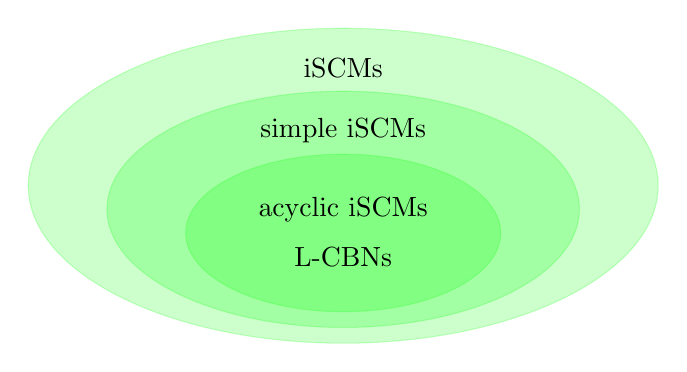
\begin{tikzpicture}
      \begin{scope}
%        \draw[draw=green,fill=green,opacity=0.2] (0,0) ellipse (1.5cm and 0.5cm);
        \draw[draw=green,fill=green,opacity=0.2] (0,0.3) ellipse (2cm and 1cm);
        \draw[draw=green,fill=green,opacity=0.2] (0,0.6) ellipse (3cm and 1.5cm);
        \draw[draw=green,fill=green,opacity=0.2] (0,0.9) ellipse (4cm and 2cm);
        \node at (0,0) {L-CBNs};
        \node at (0,0.6) {acyclic iSCMs};
        \node at (0,1.6) {simple iSCMs};
        \node at (0,2.4) {iSCMs};
      \end{scope}
  \end{tikzpicture}}

  \bigskip
  \begin{itemize}
    \item L-CBNs are interventionally equivalent to acyclic iSCMs (see Proposition~\ref{prp:interventional_equivalence_cbn_scm}).
    \item Simple iSCMs are more expressive than acyclic iSCMs (or L-CBNs), because they
      can model causal cycles due to (weak) feedback loops.
    \item iSCMs are even more expressive, but also much more complicated to work with.
  \end{itemize}
\end{frame}

\begin{frame}{Interventional equivalence of acyclic iSCMs and L-CBNs}
  \begin{Def}[Informal version of \ref{def:interventional_equivalence_cbn_scm}]
    An iSCM and an L-CBN are interventionally equivalent w.r.t.\ a subset of variables if all their intervened Markov kernels have the same marginal on this subset.
  \end{Def}
  \begin{Prp}[\ref{prp:interventional_equivalence_cbn_scm}]
  \begin{enumerate}
%    \item Given an acyclic iSCM $M$, we can construct a CBN $\tilde{M}$ that is interventionally equivalent to it (w.r.t.\ $O = V \cup W$).
    \item Given an acyclic iSCM $M$ with endogenous variables $V$ and a subset $O \subseteq V$, we can construct an L-CBN $\tilde{M}$ with observed output variables $O$ and graph $G^+(M)$ that is interventionally equivalent to $M$ w.r.t.\ $O$.
    \item Given an L-CBN $\tilde{M}$ with graph $G^+$, observed output variables $O$, and latent output variables $U$, we can construct an acyclic iSCM $M$ with causal graph $G(M) \subseteq (G^+)^{\sm U}$ that is interventionally equivalent to $\tilde{M}$ w.r.t.\ $O$.
  \end{enumerate}
  \end{Prp}
\end{frame}

\part{Cyclic iSCMs}
\frame{\partpage}

\begin{frame}{Modeling feedback loops}
  \begin{itemize}
    \item Feedback loops are often present in systems;
    \item Such systems are usually described as a system of (random) differential equations.
  \end{itemize}

  \bigskip
The \emph{equilibrium} states of such systems can sometimes be causally modelled by a (cyclic) iSCM.

\bigskip
We consider two examples:
  \begin{enumerate}
    \item Damped coupled harmonic oscillator (simple iSCM)
    \item Price-supply-demand (non-simple SCM)
  \end{enumerate}
and prove that cyclic iSCMs are simple if the causal mechanisms are sufficiently weak and smooth.
\end{frame}

\begin{frame}{Example I: Damped Coupled Harmonic Oscillator}
  \centerline{\scalebox{0.8}{\begin{tikzpicture}
    \begin{scope}
      \fill[pattern=north east lines,draw=none] (-1,-1) rectangle (0,1);
      \draw (0,-1) -- (0,1);
      \begin{scope}[yshift=5mm]
      \node (Q1) at (2,0) {$m_1$};
      \node (Q2) at (4,0) {$m_2$};
      \node (Q3) at (6,0) {$m_3$};
      \node (Q4) at (8,0) {$m_4$};
      \node (Q5) at (10,0) {$m_5$};
      \end{scope}
      \begin{scope}[yshift=-5mm]
        \node (l0) at (1,0) {$k_0$};
        \node (l1) at (3,0) {$k_1$};
        \node (l2) at (5,0) {$k_2$};
        \node (l3) at (7,0) {$k_3$};
        \node (l4) at (9,0) {$k_4$};
        \node (l5) at (11,0) {$k_5$};
      \end{scope}
      \fill[black] (2,0) circle (.2);
      \fill[black] (4,0) circle (.2);
      \fill[black] (6,0) circle (.2);
      \fill[black] (8,0) circle (.2);
      \fill[black] (10,0) circle (.2);
      \draw (12,-1) -- (12,1);
      \fill[pattern=north east lines,draw=none] (12,-1) rectangle (13,1);
      \draw[thick,decorate,decoration={coil,aspect=0.7,amplitude=4,segment length=3mm}] (0,0) -- (2,0);
      \draw[thick,decorate,decoration={coil,aspect=0.7,amplitude=4,segment length=3mm}] (2,0) -- (4,0);
      \draw[thick,decorate,decoration={coil,aspect=0.7,amplitude=4,segment length=3mm}] (4,0) -- (6,0);
      \draw[thick,decorate,decoration={coil,aspect=0.7,amplitude=4,segment length=3mm}] (6,0) -- (8,0);
      \draw[thick,decorate,decoration={coil,aspect=0.7,amplitude=4,segment length=3mm}] (8,0) -- (10,0);
      \draw[thick,decorate,decoration={coil,aspect=0.7,amplitude=4,segment length=3mm}] (10,0) -- (12,0);
      \node at (0,1.3) {\tiny $Q_0$};
      \node at (12,1.3) {\tiny $Q_6$};
    \end{scope}
  \end{tikzpicture}}}

Dynamics:
$$ \frac{d^2Q_i}{dt^2} = \frac{k_i}{m_i} (Q_{i+1} - Q_i - \ell_i) + \frac{k_{i-1}}{m_i} (Q_{i-1} - Q_i + \ell_{i-1}) -\frac{b_i}{m_i} \frac{dQ_i}{dt} \qquad i=1,\dots,d.  $$
At equilibrium (set $\frac{d^2Q_i}{dt^2} = \frac{d Q_i}{dt} = 0$ and solve each equation for $Q_i$):
$$Q_i = \frac{k_i(Q_{i+1} - \ell_i) + k_{i-1}(Q_{i-1}+\ell_{i-1})}{k_i + k_{i-1}} \qquad i=1,\dots,d.$$

  \centerline{\scalebox{0.8}{\begin{tikzpicture}
    \begin{scope}[yshift=-3cm]
      \node[varc] (Q0) at (0,0) {$Q_0$};
      \node[var] (Q1) at (2,0) {$Q_1$};
      \node[var] (Q2) at (4,0) {$Q_2$};
      \node[var] (Q3) at (6,0) {$Q_3$};
      \node[var] (Q4) at (8,0) {$Q_4$};
      \node[var] (Q5) at (10,0) {$Q_5$};
      \node[varc] (Q6) at (12,0) {$Q_6$};
      \node[varc] (K0) at (1,1) {$k_0$};
      \node[varc] (K1) at (3,1) {$k_1$};
      \node[varc] (K2) at (5,1) {$k_2$};
      \node[varc] (K3) at (7,1) {$k_3$};
      \node[varc] (K4) at (9,1) {$k_4$};
      \node[varc] (K5) at (11,1) {$k_5$};
      \node[varc] (L0) at (1,-1) {$\ell_0$};
      \node[varc] (L1) at (3,-1) {$\ell_1$};
      \node[varc] (L2) at (5,-1) {$\ell_2$};
      \node[varc] (L3) at (7,-1) {$\ell_3$};
      \node[varc] (L4) at (9,-1) {$\ell_4$};
      \node[varc] (L5) at (11,-1) {$\ell_5$};
      \draw[arr] (Q0) to (Q1);
      \draw[arr,bend left=20] (Q1) to (Q2);
      \draw[arr,bend left=20] (Q2) to (Q3);
      \draw[arr,bend left=20] (Q3) to (Q4);
      \draw[arr,bend left=20] (Q4) to (Q5);
      \draw[arr,bend left=20] (Q5) to (Q4);
      \draw[arr,bend left=20] (Q4) to (Q3);
      \draw[arr,bend left=20] (Q3) to (Q2);
      \draw[arr,bend left=20] (Q2) to (Q1);
      \draw[arr] (Q6) to (Q5);
      \draw[arr] (K0) -- (Q1);
      \draw[arr] (K1) -- (Q1);
      \draw[arr] (K1) -- (Q2);
      \draw[arr] (K2) -- (Q2);
      \draw[arr] (K2) -- (Q3);
      \draw[arr] (K3) -- (Q3);
      \draw[arr] (K3) -- (Q4);
      \draw[arr] (K4) -- (Q4);
      \draw[arr] (K4) -- (Q5);
      \draw[arr] (K5) -- (Q5);
      \draw[arr] (L0) -- (Q1);
      \draw[arr] (L1) -- (Q1);
      \draw[arr] (L1) -- (Q2);
      \draw[arr] (L2) -- (Q2);
      \draw[arr] (L2) -- (Q3);
      \draw[arr] (L3) -- (Q3);
      \draw[arr] (L3) -- (Q4);
      \draw[arr] (L4) -- (Q4);
      \draw[arr] (L4) -- (Q5);
      \draw[arr] (L5) -- (Q5);
  \end{scope}
  \end{tikzpicture}}}
\end{frame}

\begin{frame}{Example II: Price, supply and demand}
  \begin{topalignedcolumn}{0.65\linewidth}
  \begin{description}
     \item[$D$] demand of a quantity of a product
     \item[$S$] supply of a quantity of a product
     \item[$R$] price of the product
  \end{description}
  \end{topalignedcolumn}\hfill%
  \begin{topalignedcolumn}{0.3\linewidth}
    \scalebox{0.8}{\begin{tikzpicture}
%      \node at (-2.5,2) {(c)};
    \node[var] (ED) at (1.5,0) {$E_D$};
    \node[var] (D) at (1.5,-1) {$D$};
    \node[var] (ES) at (-1.5,0) {$E_S$};
    \node[var] (S) at (-1.5,-1) {$S$};
    \node[var] (P) at (0,-1) {$R$};
    \draw[arr, bend left=20] (P) edge (S);
    \draw[arr, bend left=20] (P) edge (D);
    \draw[arr, bend left=20] (S) edge (P);
    \draw[arr, bend left=20] (D) edge (P);
    \draw[arr] (ED) to (D);
    \draw[arr] (ES) to (S);
    \draw[arr] (P)  to [out=62,in=118,looseness=4.4] (P);
    \end{tikzpicture}}
  \end{topalignedcolumn}

  \medskip
  Market dynamics:
$$\begin{aligned}
    D &= \beta_D R + E_D \\
    S &= \beta_S R + E_S \\
    \frac{dR}{dt} &= D - S,
  \end{aligned}$$
  At equilibrium ($\frac{dR}{dt}=0$) we get an SCM with causal mechanism:
$$
  \begin{aligned}
    f_D(d,s,r,e_D,e_S) &:= \beta_D r + e_D \\
    f_S(d,s,r,e_D,e_S) &:= \beta_S r + e_S \\
    f_P(d,s,r,e_D,e_S) &:= r + (d - s).
  \end{aligned}
$$
  Note the self-cycle at $R$!
\end{frame}

\begin{frame}{More simple iSCMs}
  iSCMs are simple if the causal mechanisms are sufficiently weak/smooth.
  \begin{Prp}[\ref{prp:simple_scm_contraction}]
  Let $M = \lt \Sin, \Send, \Srnd, \CX, P, f \rt$ be an iSCM with real-valued endogenous variables.
  If for each subset $U \subseteq \Send$, and for all values $\xW\in\CXW$, $\xJ \in \CXJ$, $x_{V\sm U} \in \CX_{V\sm U}$, the mapping
  \begin{equation*}
  \CX_U \to \CX_U : x_U \mapsto f(\xJ,x_{V\sm U},x_U,\xW)
  \end{equation*}
  is Lipschitz continuous with Lipschitz constant $L_U(\xJ,x_{V\sm U},\xW) < 1$ with respect to some norm $||\cdot||$, then $M$ is simple.
\end{Prp}
\begin{proof}
  Application of Banach's fixed point theorem.
\end{proof}
\end{frame}

\begin{frame}{Sampling from simple iSCMs}
Simple iSCMs satisfying the assumption Proposition~\ref{prp:simple_scm_contraction} can be sampled from easily.
\begin{Rem}
   The solution to 
  $$x_U = f(\xJ,x_{V\sm U},x_U,\xW)$$
can be obtained by iterating the updates
  $$x_U^{(n+1)} = f(\xJ,x_{V\sm U},x_U^{(n)},\xW)$$
until convergence.
\end{Rem}
\end{frame}

